\begin{frame}[plain,t]
  {Digression: This presentation is created by Beamer}

  \begin{beamercolorbox}[rounded=true, center, shadow=true,wd=\linewidth]{frametitle}
    Beamer is A LaTeX class for producing presentations and slides
  \end{beamercolorbox}
  https://github.com/josephwright/beamer

  \begin{beamercolorbox}[rounded=true, center, shadow=true,wd=\linewidth]{frametitle}
    How install Beamer
  \end{beamercolorbox}
  If you have texlive, Beamer is already.

  \begin{beamercolorbox}[rounded=true, center, shadow=true,wd=\linewidth]{frametitle}
    My source codes
  \end{beamercolorbox}

  This presentation source place on
  
  https://github.com/forno/three\_min\_demo


\end{frame}

\begin{frame}[plain,t]
  {What do you need for deep learning works with CUDA}
  %%%Image area
  %\begin{minipage}[t]{\linewidth}
  %    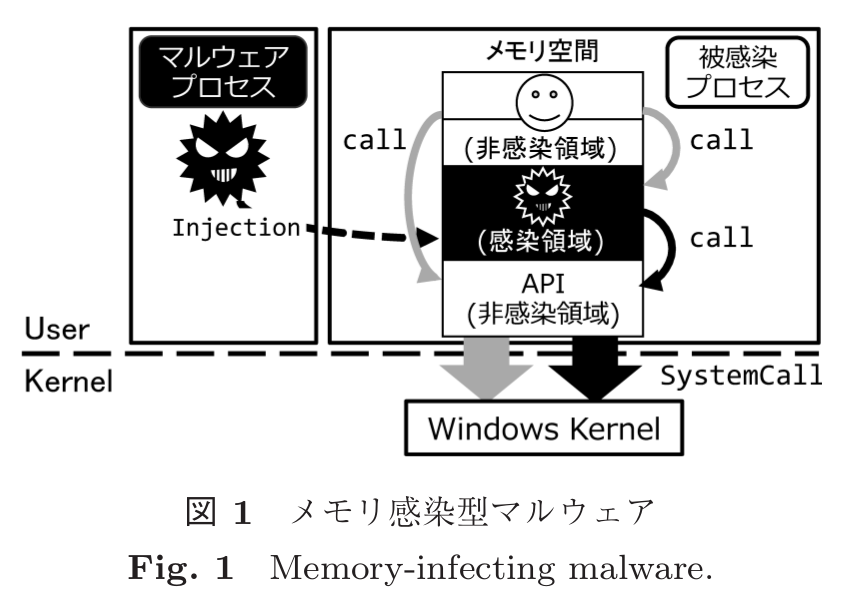
\includegraphics[height=0.15\textheight,keepaspectratio]{img/Target.png}
  %    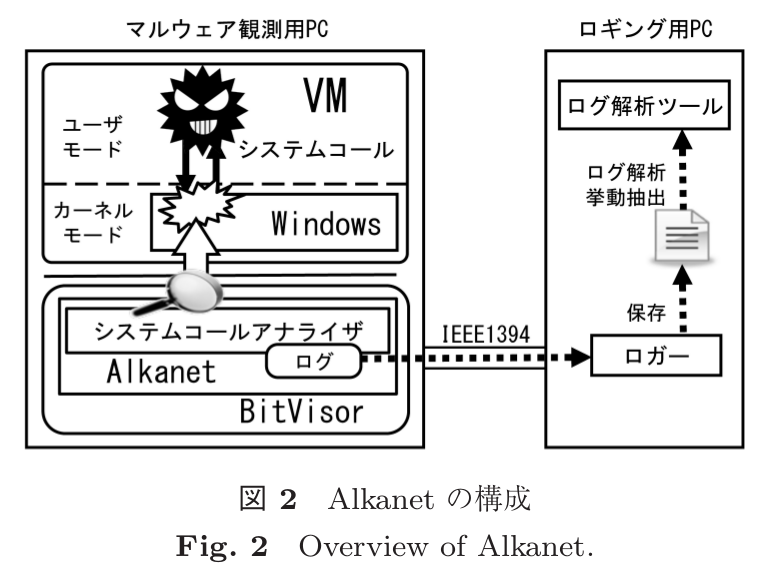
\includegraphics[height=0.15\textheight,keepaspectratio]{img/SystemOverview.png}
  %    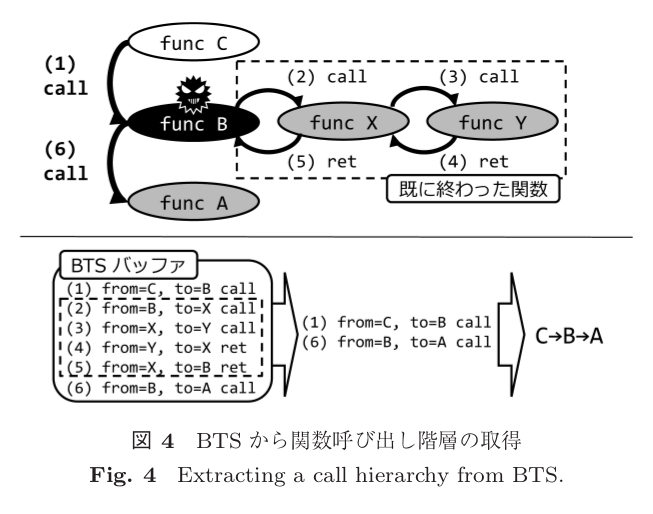
\includegraphics[height=0.15\textheight,keepaspectratio]{img/BTS.png}
  %    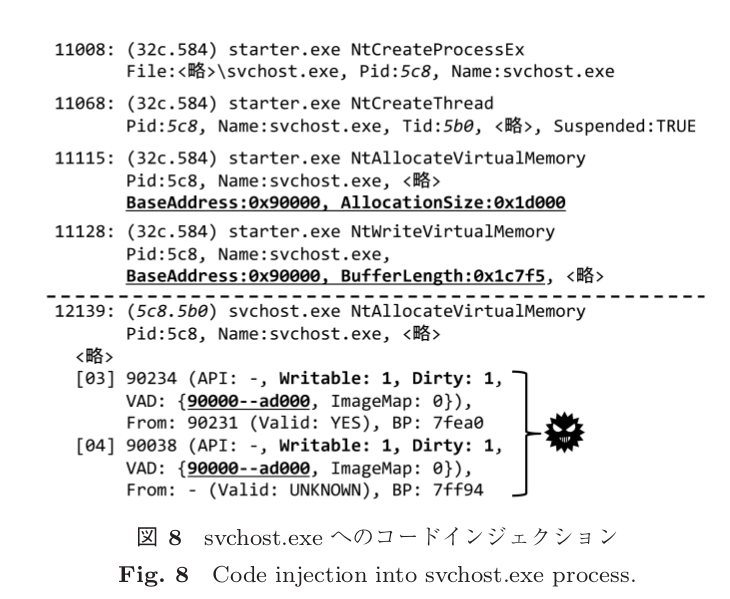
\includegraphics[height=0.15\textheight,keepaspectratio]{img/Result.png}
  %\end{minipage}

  %%%Text area
  \begin{multicols}{2}
    \begin{beamercolorbox}[rounded=true, center, shadow=true,wd=\linewidth]{frametitle}
      Device needs
    \end{beamercolorbox}
    cuDNN require GPU which have capability 3.0 or higher.

    \begin{beamercolorbox}[rounded=true, center, shadow=true,wd=\linewidth]{frametitle}
      Problem
    \end{beamercolorbox}
    High cost devices for a person

    \newpage
    \begin{beamercolorbox}[rounded=true, center, shadow=true,wd=\linewidth]{frametitle}
      Software needs
    \end{beamercolorbox}
    \begin{itemize}
      \item Apache MXNet
      \item Caffe
      \item Caffe2
      \item Chainer
      \item Gluon
      \item Keras
      \item Microsoft Cognitive Toolkit
      \item OpenPose
      \item PyTorch
      \item TensorFlow
      \item Theano
      \item Torch
    \end{itemize}

    \begin{beamercolorbox}[rounded=true, center, shadow=true,wd=\linewidth]{frametitle}
      Problem
    \end{beamercolorbox}
    Too many software and frameworks
  \end{multicols}
\end{frame}

\begin{frame}[plain,t]
  {AWS Deep Learning AMI}

  \begin{beamercolorbox}[rounded=true, center, shadow=true,wd=\linewidth]{frametitle}
    Simple way
  \end{beamercolorbox}
  Most simple method:

  \begin{enumerate}
    \item Create EC2 general-purpose GPU instance with Deep Learning AMI with Conda
    \item Run `source activate tensorflow\_p36`
    \item Run `jupyter notebook --ip='*'`
    \item Access to jupyter server
  \end{enumerate}

  You can use some deep learning tools!

  \begin{beamercolorbox}[rounded=true, center, shadow=true,wd=\linewidth]{frametitle}
    Specification of machine
  \end{beamercolorbox}

  On p3.2xlarge instance
  \begin{itemize}
    \item GPU: NVIDIA Tesla V100 GPU : x1
    \item vCPU: 8 : It means 8 cores.
    \item ECU: 23.5 : 1 ECU mean the same spec of 1.0-1.2 GHz 2007 Opteron.
    \item Memory: 61 GiB
    \item Cost: \$ $3.06 / 1$ hour
  \end{itemize}
\end{frame}
